% Options for packages loaded elsewhere
\PassOptionsToPackage{unicode}{hyperref}
\PassOptionsToPackage{hyphens}{url}
\PassOptionsToPackage{dvipsnames,svgnames,x11names}{xcolor}
%
\documentclass[
  12pt]{article}

\usepackage{amsmath,amssymb}
\usepackage{iftex}
\ifPDFTeX
  \usepackage[T1]{fontenc}
  \usepackage[utf8]{inputenc}
  \usepackage{textcomp} % provide euro and other symbols
\else % if luatex or xetex
  \usepackage{unicode-math}
  \defaultfontfeatures{Scale=MatchLowercase}
  \defaultfontfeatures[\rmfamily]{Ligatures=TeX,Scale=1}
\fi
\usepackage{lmodern}
\ifPDFTeX\else  
    % xetex/luatex font selection
\fi
% Use upquote if available, for straight quotes in verbatim environments
\IfFileExists{upquote.sty}{\usepackage{upquote}}{}
\IfFileExists{microtype.sty}{% use microtype if available
  \usepackage[]{microtype}
  \UseMicrotypeSet[protrusion]{basicmath} % disable protrusion for tt fonts
}{}
\makeatletter
\@ifundefined{KOMAClassName}{% if non-KOMA class
  \IfFileExists{parskip.sty}{%
    \usepackage{parskip}
  }{% else
    \setlength{\parindent}{0pt}
    \setlength{\parskip}{6pt plus 2pt minus 1pt}}
}{% if KOMA class
  \KOMAoptions{parskip=half}}
\makeatother
\usepackage{xcolor}
\setlength{\emergencystretch}{3em} % prevent overfull lines
\setcounter{secnumdepth}{5}
% Make \paragraph and \subparagraph free-standing
\makeatletter
\ifx\paragraph\undefined\else
  \let\oldparagraph\paragraph
  \renewcommand{\paragraph}{
    \@ifstar
      \xxxParagraphStar
      \xxxParagraphNoStar
  }
  \newcommand{\xxxParagraphStar}[1]{\oldparagraph*{#1}\mbox{}}
  \newcommand{\xxxParagraphNoStar}[1]{\oldparagraph{#1}\mbox{}}
\fi
\ifx\subparagraph\undefined\else
  \let\oldsubparagraph\subparagraph
  \renewcommand{\subparagraph}{
    \@ifstar
      \xxxSubParagraphStar
      \xxxSubParagraphNoStar
  }
  \newcommand{\xxxSubParagraphStar}[1]{\oldsubparagraph*{#1}\mbox{}}
  \newcommand{\xxxSubParagraphNoStar}[1]{\oldsubparagraph{#1}\mbox{}}
\fi
\makeatother


\providecommand{\tightlist}{%
  \setlength{\itemsep}{0pt}\setlength{\parskip}{0pt}}\usepackage{longtable,booktabs,array}
\usepackage{calc} % for calculating minipage widths
% Correct order of tables after \paragraph or \subparagraph
\usepackage{etoolbox}
\makeatletter
\patchcmd\longtable{\par}{\if@noskipsec\mbox{}\fi\par}{}{}
\makeatother
% Allow footnotes in longtable head/foot
\IfFileExists{footnotehyper.sty}{\usepackage{footnotehyper}}{\usepackage{footnote}}
\makesavenoteenv{longtable}
\usepackage{graphicx}
\makeatletter
\def\maxwidth{\ifdim\Gin@nat@width>\linewidth\linewidth\else\Gin@nat@width\fi}
\def\maxheight{\ifdim\Gin@nat@height>\textheight\textheight\else\Gin@nat@height\fi}
\makeatother
% Scale images if necessary, so that they will not overflow the page
% margins by default, and it is still possible to overwrite the defaults
% using explicit options in \includegraphics[width, height, ...]{}
\setkeys{Gin}{width=\maxwidth,height=\maxheight,keepaspectratio}
% Set default figure placement to htbp
\makeatletter
\def\fps@figure{htbp}
\makeatother

\addtolength{\oddsidemargin}{-.5in}%
\addtolength{\evensidemargin}{-1in}%
\addtolength{\textwidth}{1in}%
\addtolength{\textheight}{1.7in}%
\addtolength{\topmargin}{-1in}%
\makeatletter
\@ifpackageloaded{caption}{}{\usepackage{caption}}
\AtBeginDocument{%
\ifdefined\contentsname
  \renewcommand*\contentsname{Tabla de contenidos}
\else
  \newcommand\contentsname{Tabla de contenidos}
\fi
\ifdefined\listfigurename
  \renewcommand*\listfigurename{Listado de Figuras}
\else
  \newcommand\listfigurename{Listado de Figuras}
\fi
\ifdefined\listtablename
  \renewcommand*\listtablename{Listado de Tablas}
\else
  \newcommand\listtablename{Listado de Tablas}
\fi
\ifdefined\figurename
  \renewcommand*\figurename{Figura}
\else
  \newcommand\figurename{Figura}
\fi
\ifdefined\tablename
  \renewcommand*\tablename{Tabla}
\else
  \newcommand\tablename{Tabla}
\fi
}
\@ifpackageloaded{float}{}{\usepackage{float}}
\floatstyle{ruled}
\@ifundefined{c@chapter}{\newfloat{codelisting}{h}{lop}}{\newfloat{codelisting}{h}{lop}[chapter]}
\floatname{codelisting}{Listado}
\newcommand*\listoflistings{\listof{codelisting}{Listado de Listados}}
\makeatother
\makeatletter
\makeatother
\makeatletter
\@ifpackageloaded{caption}{}{\usepackage{caption}}
\@ifpackageloaded{subcaption}{}{\usepackage{subcaption}}
\makeatother

\ifLuaTeX
\usepackage[bidi=basic]{babel}
\else
\usepackage[bidi=default]{babel}
\fi
\babelprovide[main,import]{spanish}
% get rid of language-specific shorthands (see #6817):
\let\LanguageShortHands\languageshorthands
\def\languageshorthands#1{}
\ifLuaTeX
  \usepackage{selnolig}  % disable illegal ligatures
\fi
\usepackage[]{natbib}
\bibliographystyle{agsm}
\usepackage{bookmark}

\IfFileExists{xurl.sty}{\usepackage{xurl}}{} % add URL line breaks if available
\urlstyle{same} % disable monospaced font for URLs
\hypersetup{
  pdftitle={1. Cantidad proyectada para 2024 en base a la poblacion de 2020 y su taza de crecimiento},
  pdfauthor={Andres Humberto Chirinos Lizondo},
  pdflang={es},
  pdfkeywords={Unidades Educativas, Crecimiento},
  colorlinks=true,
  linkcolor={blue},
  filecolor={Maroon},
  citecolor={Blue},
  urlcolor={Blue},
  pdfcreator={LaTeX via pandoc}}



\begin{document}


\def\spacingset#1{\renewcommand{\baselinestretch}%
{#1}\small\normalsize} \spacingset{1}


%%%%%%%%%%%%%%%%%%%%%%%%%%%%%%%%%%%%%%%%%%%%%%%%%%%%%%%%%%%%%%%%%%%%%%%%%%%%%%

\date{octubre 17, 2024}
\title{\bf 1. Cantidad proyectada para 2024 en base a la poblacion de
2020 y su taza de crecimiento}
\author{
Andres Humberto Chirinos Lizondo\\
Carrera de Estadística - UMSA\\
}
\maketitle

\bigskip
\bigskip
\begin{abstract}
Breve resumen de las proyecciones de la cantidad de unidades educativas
y estudiantes para el año 2024 en base a datos del año 2020.
\end{abstract}

\noindent%
{\it Keywords:} Unidades Educativas, Crecimiento
\vfill

\newpage
\spacingset{1.9} % DON'T change the spacing!


\[
c_{2024} = c_{2020} + 4(a)
\]

Donde.

\begin{itemize}
\item
  \(c_{2024}\) es la cantidad de estudiantes para 2024
\item
  \(c_{2020}\) es la cantidad de estudiantes para 2020
\item
  \(a\) es el crecimiento anual de estudiantes
\end{itemize}

\textsubscript{Fuente:
\href{https://sociest.github.io/ue-report/index.ipynb.html}{Cuaderno de
Artículo}}

\begin{figure}[H]

\centering{

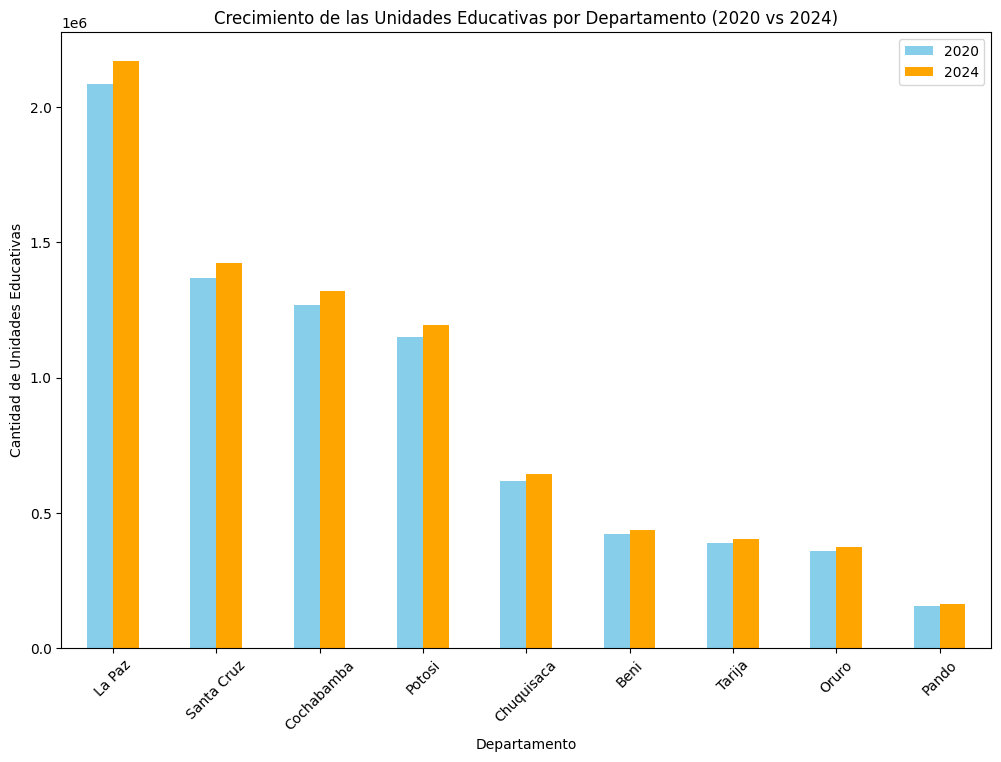
\includegraphics{index_files/figure-pdf/fig-crec2024-output-1.png}

}

\caption{\label{fig-crec2024}Crecimiento de las Unidades Educativas por
Departamento (2020 vs 2024)}

\end{figure}%

\textsubscript{Fuente:
\href{https://sociest.github.io/ue-report/index.ipynb.html}{Cuaderno de
Artículo}}

2. Cantidad de Unidades Educativas por departamento

\textsubscript{Fuente:
\href{https://sociest.github.io/ue-report/index.ipynb.html}{Cuaderno de
Artículo}}

\begin{figure}[H]

\centering{

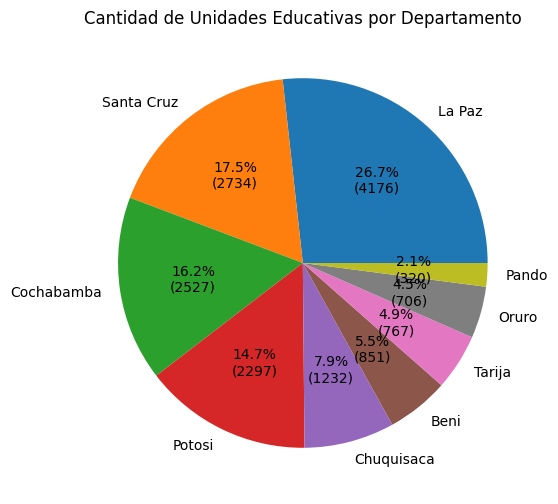
\includegraphics{index_files/figure-pdf/fig-rept2024-output-1.png}

}

\caption{\label{fig-rept2024}Conteo de unidades educativas por
departamento}

\end{figure}%

\textsubscript{Fuente:
\href{https://sociest.github.io/ue-report/index.ipynb.html}{Cuaderno de
Artículo}}

\subsection{Comentarios sobre el gráfico de unidades educativas en
Bolivia}\label{comentarios-sobre-el-gruxe1fico-de-unidades-educativas-en-bolivia}

El gráfico anterior muestra la distribución de las unidades educativas
en Bolivia. Las áreas están coloreadas según la cantidad de unidades
educativas presentes en cada municipio. Los municipios con más unidades
educativas están representados con colores más oscuros, mientras que los
municipios con menos unidades educativas están representados con colores
más claros.

\subsubsection{Observaciones:}\label{observaciones}

\begin{itemize}
\tightlist
\item
  La mayoría de las unidades educativas se concentran en los
  departamentos más poblados.
\item
  Existen municipios que no tienen unidades educativas asignadas, lo
  cual se refleja en el color más claro.
\item
  Este análisis permite identificar las áreas con mayor necesidad de
  infraestructura educativa.
\end{itemize}

\subsection{Unidades educativas sin municipio
asignado}\label{unidades-educativas-sin-municipio-asignado}

A continuación se muestra una tabla con las unidades educativas que no
tienen un municipio asignado. Esto puede deberse a errores en los datos
o a la falta de información geográfica precisa

\textsubscript{Fuente:
\href{https://sociest.github.io/ue-report/index.ipynb.html}{Cuaderno de
Artículo}}

3. Resumen de cantidad de Unidades Educativas por Departamento,
Provincia y Municipio desagregado

\textsubscript{Fuente:
\href{https://sociest.github.io/ue-report/index.ipynb.html}{Cuaderno de
Artículo}}

\begin{longtable}[]{@{}lllll@{}}
\toprule\noalign{}
& c\_ut & Cantidad de Estudiantes & Cantidad de Colegios & ratio \\
\midrule\noalign{}
\endhead
\bottomrule\noalign{}
\endlastfoot
0 & 010101 & 102215 & 195 & 524.179487 \\
1 & 010102 & 15093 & 31 & 486.870968 \\
2 & 010103 & 27007 & 50 & 540.140000 \\
3 & 010201 & 22438 & 38 & 590.473684 \\
4 & 010202 & 25621 & 44 & 582.295455 \\
... & ... & ... & ... & ... \\
330 & 090401 & 4811 & 9 & 534.555556 \\
331 & 090402 & 3586 & 8 & 448.250000 \\
332 & 090501 & 3017 & 6 & 502.833333 \\
333 & 090502 & 6835 & 17 & 402.058824 \\
334 & 090503 & 1891 & 5 & 378.200000 \\
\end{longtable}

\begin{verbatim}
520.9182046132242
70.60677697466468
\end{verbatim}

\textsubscript{Fuente:
\href{https://sociest.github.io/ue-report/index.ipynb.html}{Cuaderno de
Artículo}}

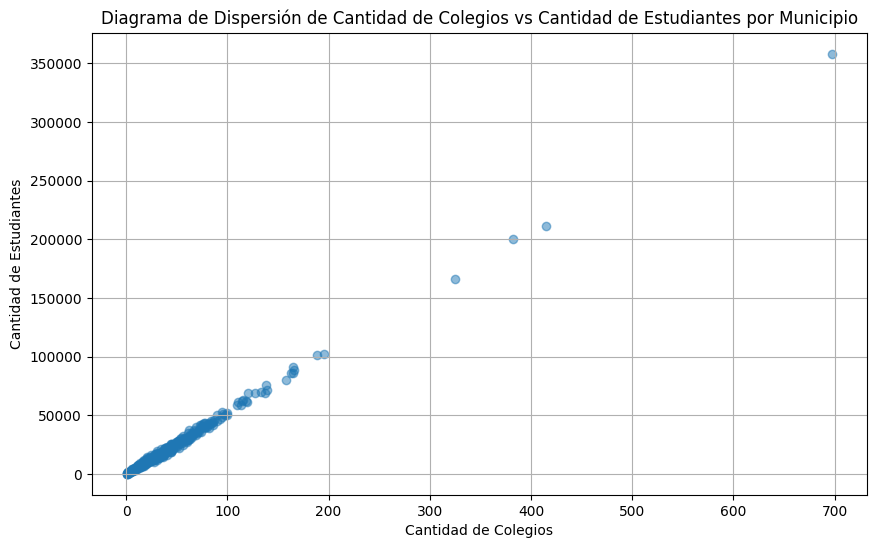
\includegraphics{index_files/figure-pdf/cell-11-output-1.png}

\textsubscript{Fuente:
\href{https://sociest.github.io/ue-report/index.ipynb.html}{Cuaderno de
Artículo}}

\begin{verbatim}
Índice de correlación: 0.9982796142756408
Promedio de estudiantes por unidad educativa: 24253.758208955223
Varianza de estudiantes por unidad educativa: 929233318.686871
\end{verbatim}

\textsubscript{Fuente:
\href{https://sociest.github.io/ue-report/index.ipynb.html}{Cuaderno de
Artículo}}

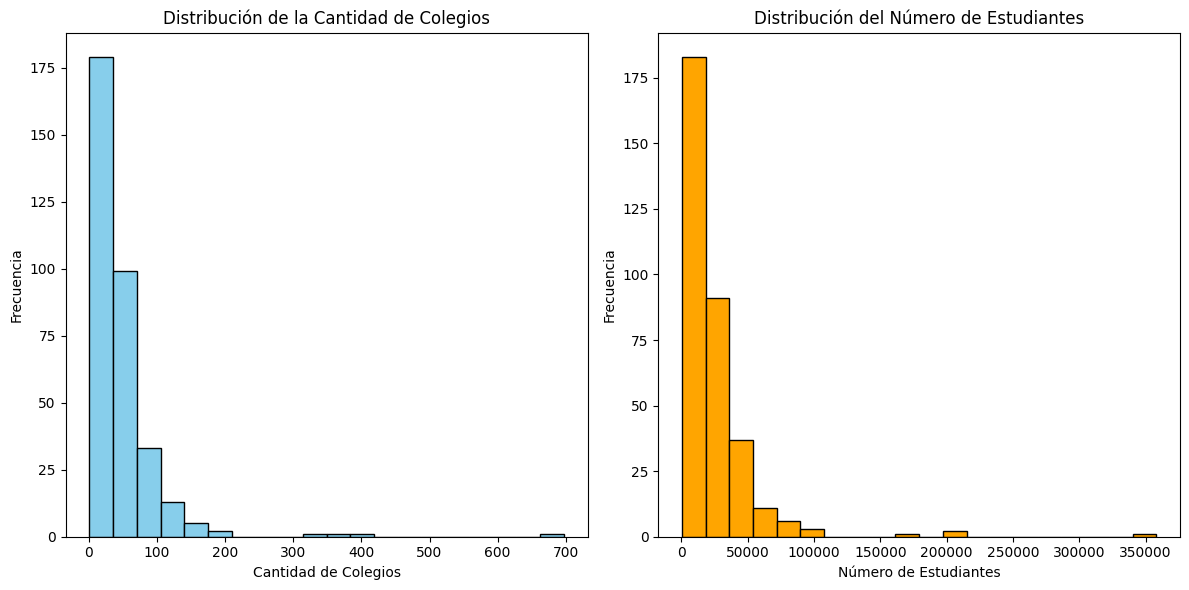
\includegraphics{index_files/figure-pdf/cell-13-output-1.png}

\textsubscript{Fuente:
\href{https://sociest.github.io/ue-report/index.ipynb.html}{Cuaderno de
Artículo}}

\begin{figure}[H]

\centering{

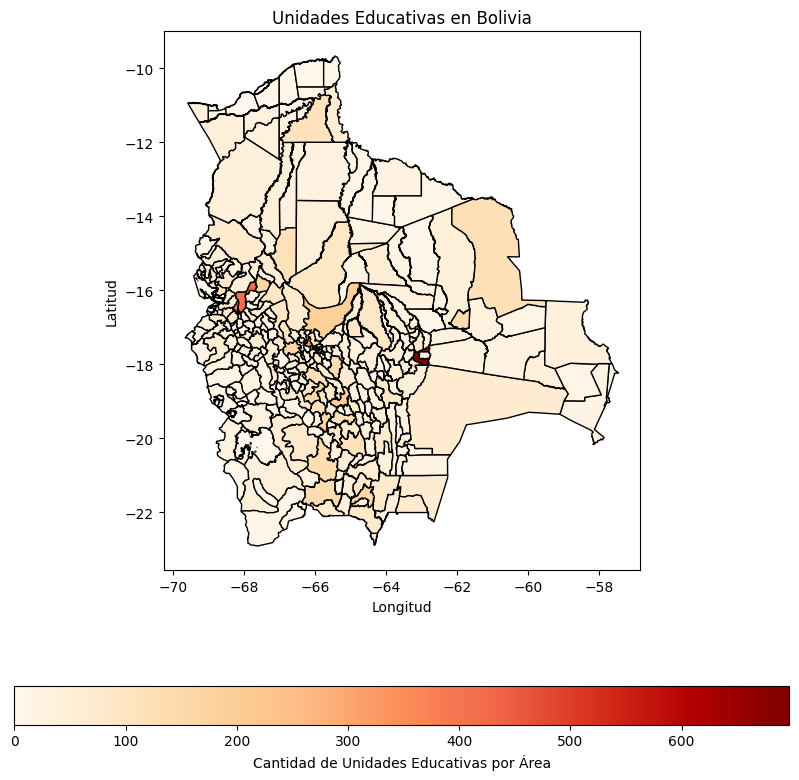
\includegraphics{index_files/figure-pdf/fig-mun2024-output-2.png}

}

\caption{\label{fig-mun2024}Conteo de unidades educativas por municipio}

\end{figure}%

\textsubscript{Fuente:
\href{https://sociest.github.io/ue-report/index.ipynb.html}{Cuaderno de
Artículo}}

\begin{figure}[H]

\centering{

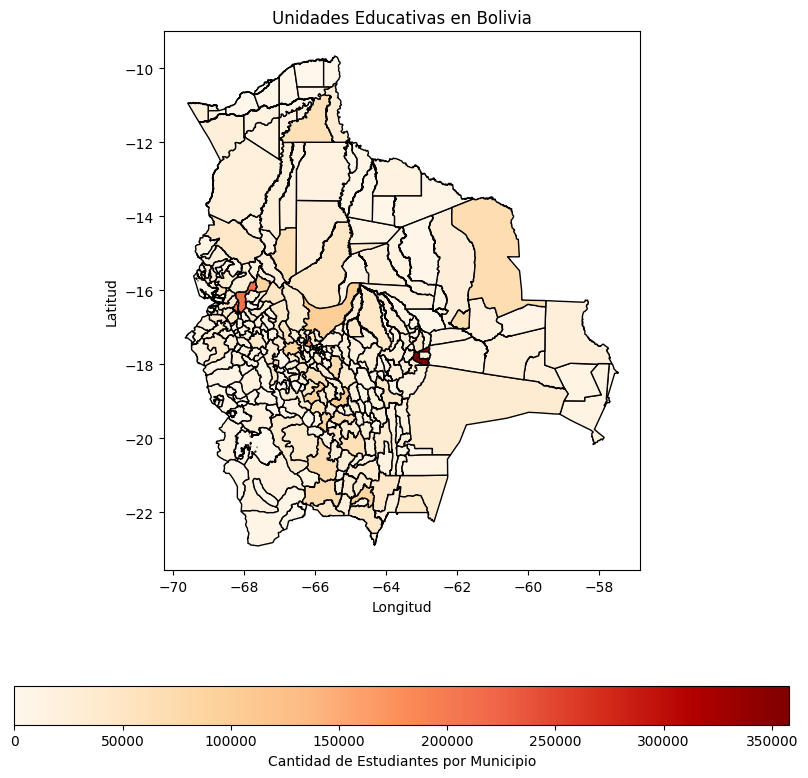
\includegraphics{index_files/figure-pdf/fig-mun2024cant-output-2.png}

}

\caption{\label{fig-mun2024cant}Conteo de estudiantes por municipio}

\end{figure}%

\textsubscript{Fuente:
\href{https://sociest.github.io/ue-report/index.ipynb.html}{Cuaderno de
Artículo}}

\section{3.2. Ordenado por tamaño}\label{ordenado-por-tamauxf1o}

\textsubscript{Fuente:
\href{https://sociest.github.io/ue-report/index.ipynb.html}{Cuaderno de
Artículo}}

\begin{longtable}[]{@{}llllll@{}}

\caption{\label{tbl-depprovmun}Cantidad de Unidades Educativas por
Departamento, Provincia y Municipio desagregado, ordenado por cantidad}

\tabularnewline

\toprule\noalign{}
& Departamento & Provincia & Municipio & CodigoINE & Cantidad de
Unidades Educativas \\
\midrule\noalign{}
\endhead
\bottomrule\noalign{}
\endlastfoot
0 & Santa Cruz & Andres Iba?ez & Santa Cruz de la Sierra & 070101 &
697 \\
1 & La Paz & Murillo & Nuestra Senora de La Paz & 020101 & 415 \\
2 & La Paz & Murillo & El Alto & 020105 & 382 \\
3 & Cochabamba & Cercado & Cochabamba & 030101 & 325 \\
4 & Chuquisaca & Oropeza & Sucre & 010101 & 195 \\
... & ... & ... & ... & ... & ... \\
333 & Oruro & Litoral & Escara & 040502 & 1 \\
334 & Oruro & Mejillones & Carangas & 041503 & 1 \\
335 & Oruro & Litoral & Yunguyo del Litoral & 040504 & 1 \\
336 & Oruro & Mejillones & La Rivera & 041501 & 1 \\
337 & La Paz & Pacajes & Nazacara de Pacajes & 020307 & 1 \\

\end{longtable}

\textsubscript{Fuente:
\href{https://sociest.github.io/ue-report/index.ipynb.html}{Cuaderno de
Artículo}}

\section{3.1. Ordenado por Departamento, Provincia y
Municipio}\label{ordenado-por-departamento-provincia-y-municipio}

\textsubscript{Fuente:
\href{https://sociest.github.io/ue-report/index.ipynb.html}{Cuaderno de
Artículo}}

\begin{longtable}[]{@{}llllll@{}}

\caption{\label{tbl-depprovmun2}Cantidad de Unidades Educativas por
Departamento, Provincia y Municipio desagregado, ordenado por Ubicación}

\tabularnewline

\toprule\noalign{}
& Departamento & Provincia & Municipio & CodigoINE & Cantidad de
Unidades Educativas \\
\midrule\noalign{}
\endhead
\bottomrule\noalign{}
\endlastfoot
0 & Beni & Cercado & San Javier & 080102 & 24 \\
1 & Beni & Cercado & Trinidad & 080101 & 75 \\
2 & Beni & General Jose Balliv & Reyes & 080301 & 49 \\
3 & Beni & General Jose Balliv & Rurrenabaque & 080304 & 36 \\
4 & Beni & General Jose Balliv & San Borja & 080302 & 119 \\
... & ... & ... & ... & ... & ... \\
333 & Tarija & Gran Chaco & Carapari & 060302 & 46 \\
334 & Tarija & Gran Chaco & Villamontes & 060303 & 63 \\
335 & Tarija & Gran Chaco & Yacuiba & 060301 & 74 \\
336 & Tarija & Mendez & Tomayapo (El Puente) & 060502 & 57 \\
337 & Tarija & Mendez & Villa San Lorenzo & 060501 & 82 \\

\end{longtable}

\textsubscript{Fuente:
\href{https://sociest.github.io/ue-report/index.ipynb.html}{Cuaderno de
Artículo}}

4. Resumen de las Unidades Educativas por Departamento, que tengan 991 y
1000 estudiantes.

\textsubscript{Fuente:
\href{https://sociest.github.io/ue-report/index.ipynb.html}{Cuaderno de
Artículo}}

\begin{longtable}[]{@{}lll@{}}
\toprule\noalign{}
& Departamento & Cantidad de Unidades Educativas \\
\midrule\noalign{}
\endhead
\bottomrule\noalign{}
\endlastfoot
0 & La Paz & 44 \\
1 & Potosi & 27 \\
2 & Cochabamba & 27 \\
3 & Santa Cruz & 22 \\
4 & Chuquisaca & 14 \\
5 & Beni & 5 \\
6 & Tarija & 5 \\
7 & Oruro & 3 \\
8 & Pando & 2 \\
\end{longtable}

\textsubscript{Fuente:
\href{https://sociest.github.io/ue-report/index.ipynb.html}{Cuaderno de
Artículo}}

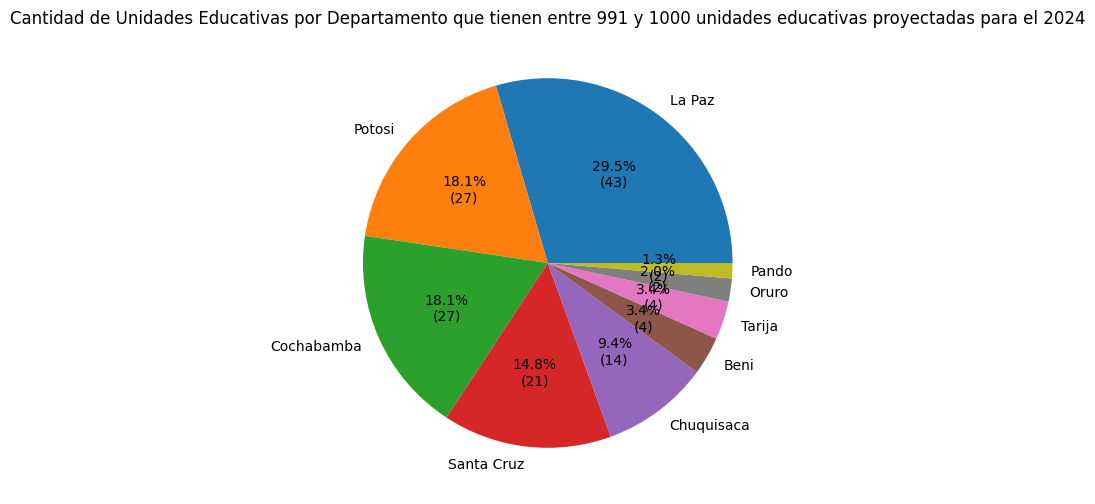
\includegraphics{index_files/figure-pdf/cell-20-output-1.png}

\textsubscript{Fuente:
\href{https://sociest.github.io/ue-report/index.ipynb.html}{Cuaderno de
Artículo}}

\section{4.1. Comparativa de Tamaño de grupo con respecto al
resto}\label{comparativa-de-tamauxf1o-de-grupo-con-respecto-al-resto}

\textsubscript{Fuente:
\href{https://sociest.github.io/ue-report/index.ipynb.html}{Cuaderno de
Artículo}}

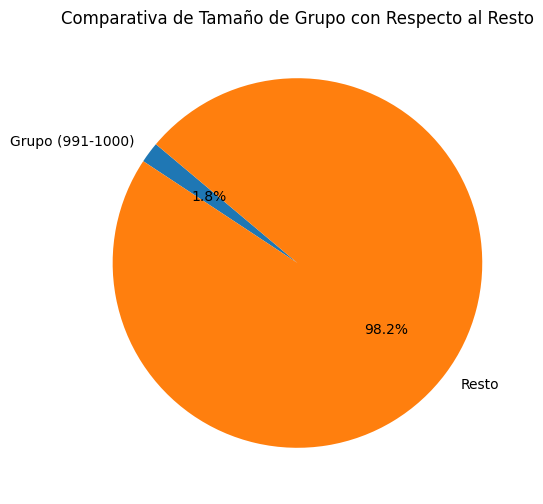
\includegraphics{index_files/figure-pdf/cell-21-output-1.png}

\textsubscript{Fuente:
\href{https://sociest.github.io/ue-report/index.ipynb.html}{Cuaderno de
Artículo}}

\section{4.2 Segmentación por
modalidad}\label{segmentaciuxf3n-por-modalidad}

\textsubscript{Fuente:
\href{https://sociest.github.io/ue-report/index.ipynb.html}{Cuaderno de
Artículo}}

\begin{longtable}[]{@{}lll@{}}
\toprule\noalign{}
& Modalidad & Cantidad de Unidades Educativas \\
\midrule\noalign{}
\endhead
\bottomrule\noalign{}
\endlastfoot
0 & Regular & 144 \\
1 & Alternativa & 4 \\
2 & Especial & 1 \\
\end{longtable}

\textsubscript{Fuente:
\href{https://sociest.github.io/ue-report/index.ipynb.html}{Cuaderno de
Artículo}}

\section{4.3 Segmentación por area}\label{segmentaciuxf3n-por-area}

\textsubscript{Fuente:
\href{https://sociest.github.io/ue-report/index.ipynb.html}{Cuaderno de
Artículo}}

\begin{longtable}[]{@{}lll@{}}
\toprule\noalign{}
& Area & Cantidad de Unidades Educativas \\
\midrule\noalign{}
\endhead
\bottomrule\noalign{}
\endlastfoot
0 & R & 121 \\
1 & U & 28 \\
\end{longtable}

\textsubscript{Fuente:
\href{https://sociest.github.io/ue-report/index.ipynb.html}{Cuaderno de
Artículo}}

5. Resumen de Area de las unidades educativas

\textsubscript{Fuente:
\href{https://sociest.github.io/ue-report/index.ipynb.html}{Cuaderno de
Artículo}}

\begin{verbatim}
area
R    12132
U     3483
Name: fid_unidad, dtype: int64
\end{verbatim}

\textsubscript{Fuente:
\href{https://sociest.github.io/ue-report/index.ipynb.html}{Cuaderno de
Artículo}}

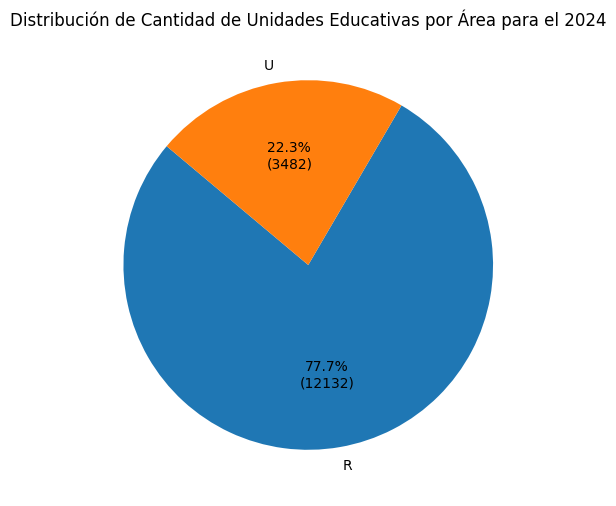
\includegraphics{index_files/figure-pdf/cell-25-output-1.png}

\textsubscript{Fuente:
\href{https://sociest.github.io/ue-report/index.ipynb.html}{Cuaderno de
Artículo}}

\begin{verbatim}
area
R    6306290
U    1818719
Name: cant_2024, dtype: int64
\end{verbatim}

\textsubscript{Fuente:
\href{https://sociest.github.io/ue-report/index.ipynb.html}{Cuaderno de
Artículo}}

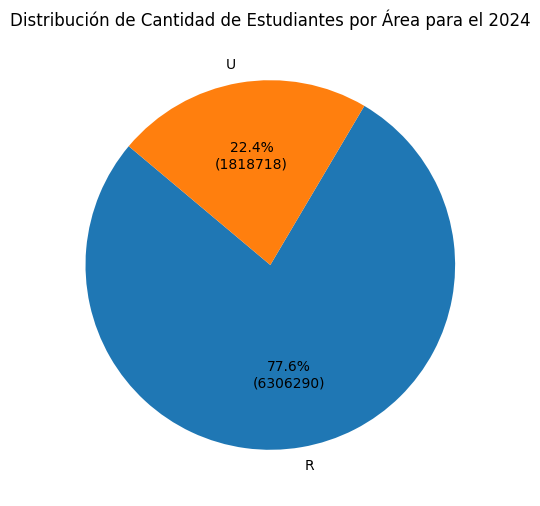
\includegraphics{index_files/figure-pdf/cell-27-output-1.png}

\textsubscript{Fuente:
\href{https://sociest.github.io/ue-report/index.ipynb.html}{Cuaderno de
Artículo}}

6. Resumen de Modalidad de las Unidades educativas

\textsubscript{Fuente:
\href{https://sociest.github.io/ue-report/index.ipynb.html}{Cuaderno de
Artículo}}

\begin{verbatim}
modalidad
Regular        15081
Alternativa      506
Especial          28
Name: fid_unidad, dtype: int64
\end{verbatim}

\textsubscript{Fuente:
\href{https://sociest.github.io/ue-report/index.ipynb.html}{Cuaderno de
Artículo}}

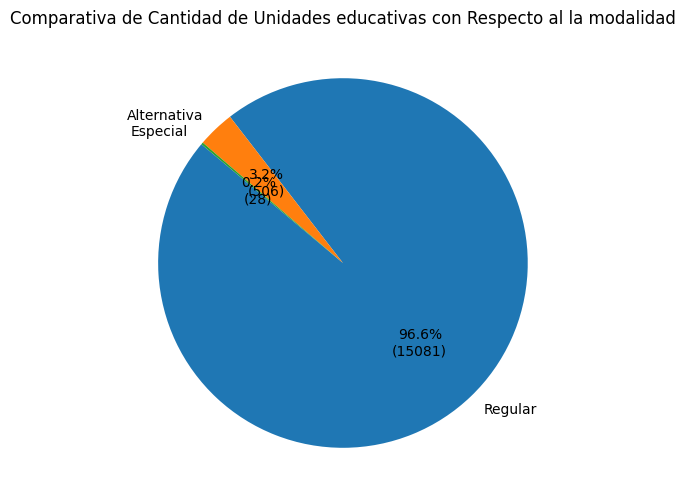
\includegraphics{index_files/figure-pdf/cell-29-output-1.png}

\textsubscript{Fuente:
\href{https://sociest.github.io/ue-report/index.ipynb.html}{Cuaderno de
Artículo}}

\begin{verbatim}
modalidad
Regular        7846094
Alternativa     265647
Especial         13268
Name: cant_2024, dtype: int64
\end{verbatim}

\textsubscript{Fuente:
\href{https://sociest.github.io/ue-report/index.ipynb.html}{Cuaderno de
Artículo}}

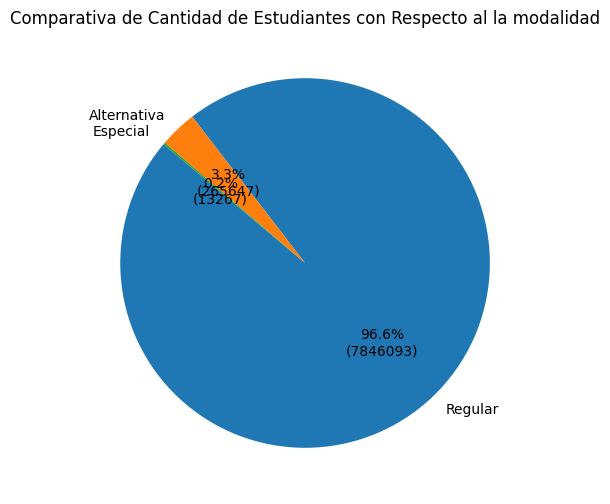
\includegraphics{index_files/figure-pdf/cell-31-output-1.png}

\textsubscript{Fuente:
\href{https://sociest.github.io/ue-report/index.ipynb.html}{Cuaderno de
Artículo}}

7. Resumen de cruce de variables

\textsubscript{Fuente:
\href{https://sociest.github.io/ue-report/index.ipynb.html}{Cuaderno de
Artículo}}

\begin{verbatim}
Conteo de unidades por modalidad y área:
modalidad    area
Regular      R       11923
             U        3158
Alternativa  U         310
             R         196
Especial     U          15
             R          13
Name: fid_unidad, dtype: int64
\end{verbatim}

\textsubscript{Fuente:
\href{https://sociest.github.io/ue-report/index.ipynb.html}{Cuaderno de
Artículo}}

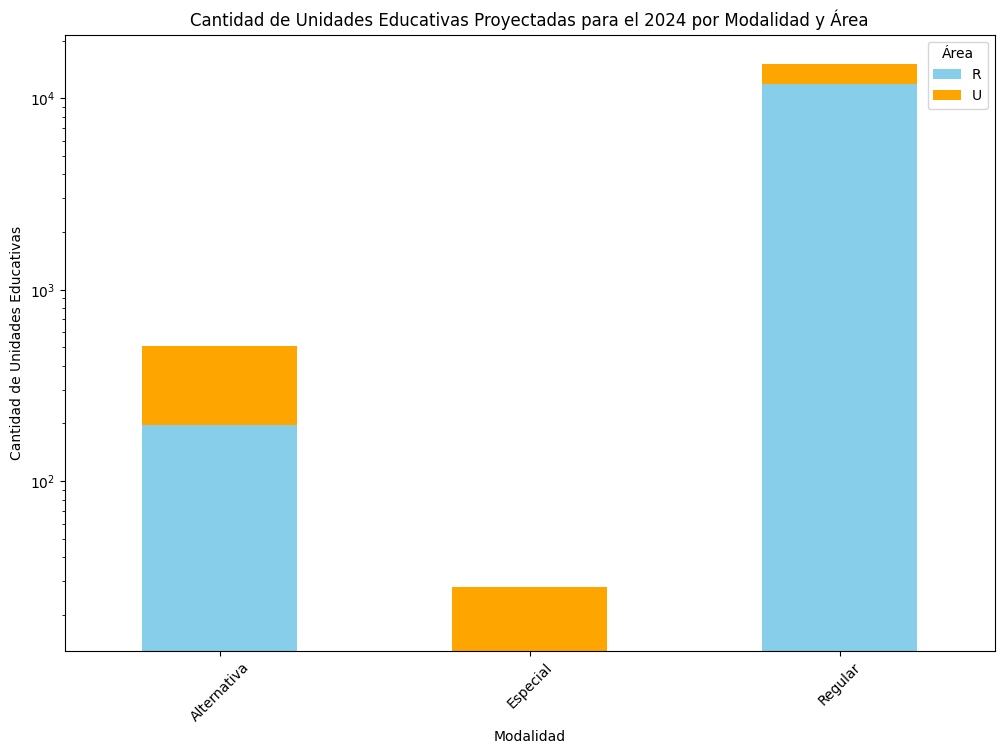
\includegraphics{index_files/figure-pdf/cell-33-output-1.png}

\textsubscript{Fuente:
\href{https://sociest.github.io/ue-report/index.ipynb.html}{Cuaderno de
Artículo}}

\begin{verbatim}

Suma de cantidad de estudiantes por modalidad y área:
modalidad    area
Regular      R       6200152
             U       1645942
Alternativa  U        164986
             R        100661
Especial     U          7791
             R          5477
Name: cant_2024, dtype: int64
\end{verbatim}

\textsubscript{Fuente:
\href{https://sociest.github.io/ue-report/index.ipynb.html}{Cuaderno de
Artículo}}

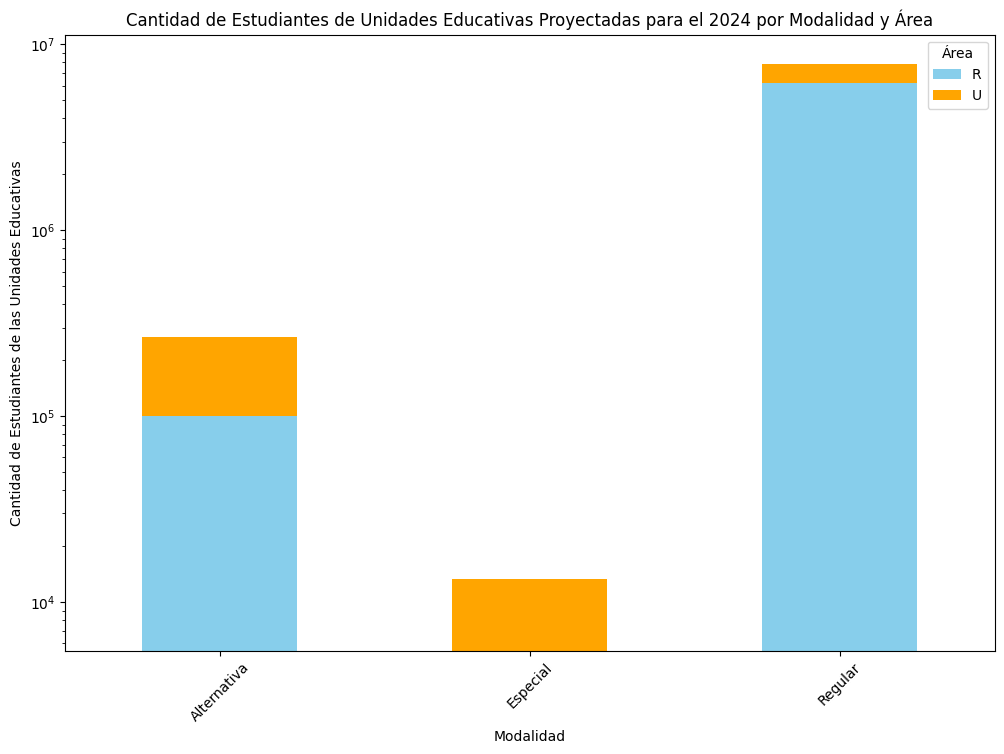
\includegraphics{index_files/figure-pdf/cell-35-output-1.png}

\textsubscript{Fuente:
\href{https://sociest.github.io/ue-report/index.ipynb.html}{Cuaderno de
Artículo}}

\begin{quote}
*Notese que esta en escala logaritmica
\end{quote}

\textsubscript{Fuente:
\href{https://sociest.github.io/ue-report/index.ipynb.html}{Cuaderno de
Artículo}}

\section*{Referencias}\label{referencias}
\addcontentsline{toc}{section}{Referencias}

\textsubscript{Fuente:
\href{https://sociest.github.io/ue-report/index.ipynb.html}{Cuaderno de
Artículo}}


  \bibliography{assets/references.bib}



\end{document}
